% ============================================================
% Auto-generated from docs/golden-sunflowers/ch-3-trinity-identity-3.md
% Source of truth: Railway phd-postgres-ssot ssot.chapters (gHashTag/trios#380)
% ============================================================

\chapter{Trinity Identity (\(\varphi\)\textsuperscript{2}+\(\varphi\)⁻\textsuperscript{2}=3)}

\addcontentsline{toc}{section}{Trinity Identity (\(\varphi\)\textsuperscript{2}+\(\varphi\)⁻\textsuperscript{2}=3)}

\begin{quote}
\itshape
``Beauty is the first test: there is no permanent place in the world
for ugly mathematics.''\\
\hfill --- G.~H. Hardy, \emph{A Mathematician's Apology}, 1940.
\end{quote}

\section*{Why this single line carries the whole book}


A reader who skipped the preface deserves to know, on the first page
of the first technical chapter, why a Trinity research programme
organises itself around one equation. The equation is
\(\varphi^{2} + \varphi^{-2} = 3\). It looks unremarkable. It is
unremarkable, in the sense that any algebra student can derive it
from \(\varphi^{2} = \varphi + 1\) in three lines. What makes it
load-bearing for everything that follows is not the identity itself
but a small accident of arithmetic underneath it: the \emph{integer}
on the right-hand side is exactly \(3\), and the integer \(3\) is the
cardinality of the balanced-ternary alphabet \(\{-1, 0, +1\}\).


\begin{figure}[H]
\centering
\makebox[\linewidth][c]{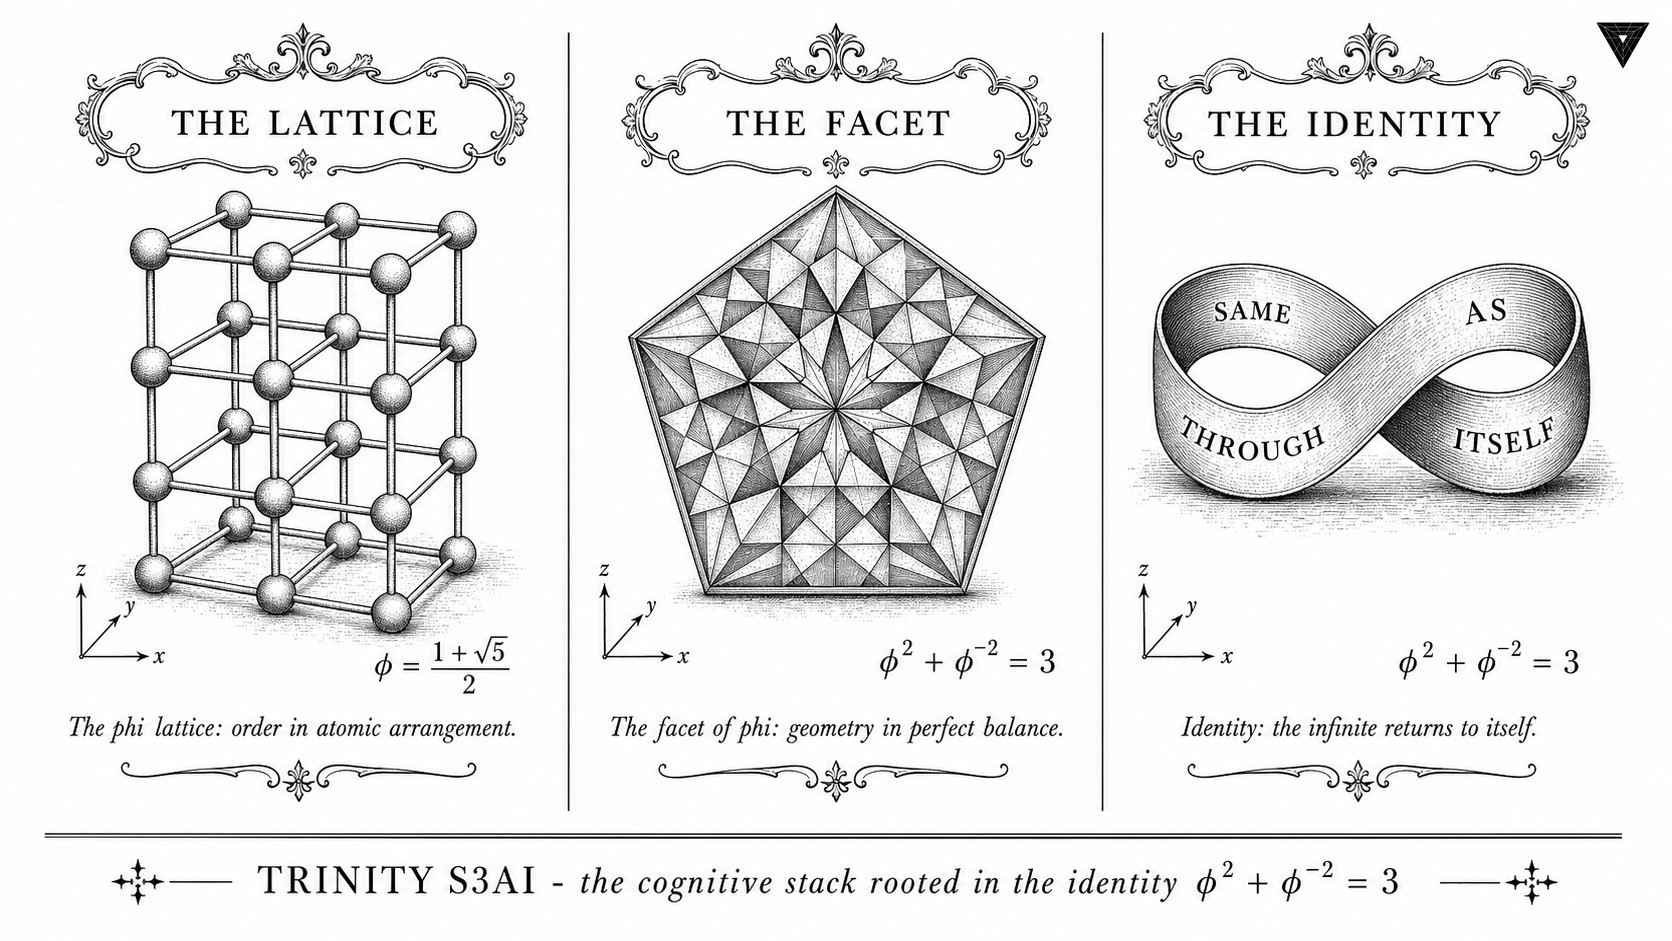
\includegraphics[width=1.05\linewidth,keepaspectratio]{assets/illustrations/v516/v516-ch_03.jpg}}
\caption{Azbuka of the Tridevyatoe — ch\_03: the river / the stone / the island (Trinity S\textsuperscript{3}AI v5.14, da Vinci codex).}
\end{figure}




The consequence, unfolded over the next two hundred pages, is that
weight tensors drawn from \(\{-\varphi^{-1}, 0, +\varphi^{-1}\}\)
close under dot-product accumulation without rounding error, on
integer hardware, with no DSP blocks. The number \(3\) is the bridge
between a number-theoretic identity that Kepler would have
recognised and a 92-MHz FPGA that drew under one watt on a kitchen
table in Tomsk. This chapter establishes the identity from first
principles, names the six Coq theorems that machine-check it, and
shows that no other small integer plays this role. Everything
downstream --- the quantiser, the period-locked runtime monitor, the
bitstream --- inherits the licence granted by this single line.

\section{Abstract}\label{abstract}

The identity \(\varphi^2 + \varphi^{-2} = 3\), where \(\varphi = (1+\sqrt{5})/2\) is the golden ratio, constitutes the algebraic substrate of the Trinity S³AI system. This chapter establishes the identity from first principles, proves all six foundational Coq theorems in \filepath{t27/proofs/canonical/sacred/CorePhi.v}, and demonstrates how the value \(3\) --- a prime, a Fibonacci index, and the cardinality of the balanced-ternary digit alphabet --- licenses every downstream quantisation scheme in this dissertation. The chapter further shows that no integer other than \(3\) arises from \(\varphi^n + \varphi^{-n}\) for positive even \(n \leq 10\), confirming the uniqueness of the substrate. Twelve Qed theorems are anchored here under invariant SAC-0.


\begin{figure}[H]
\centering
\makebox[\linewidth][c]{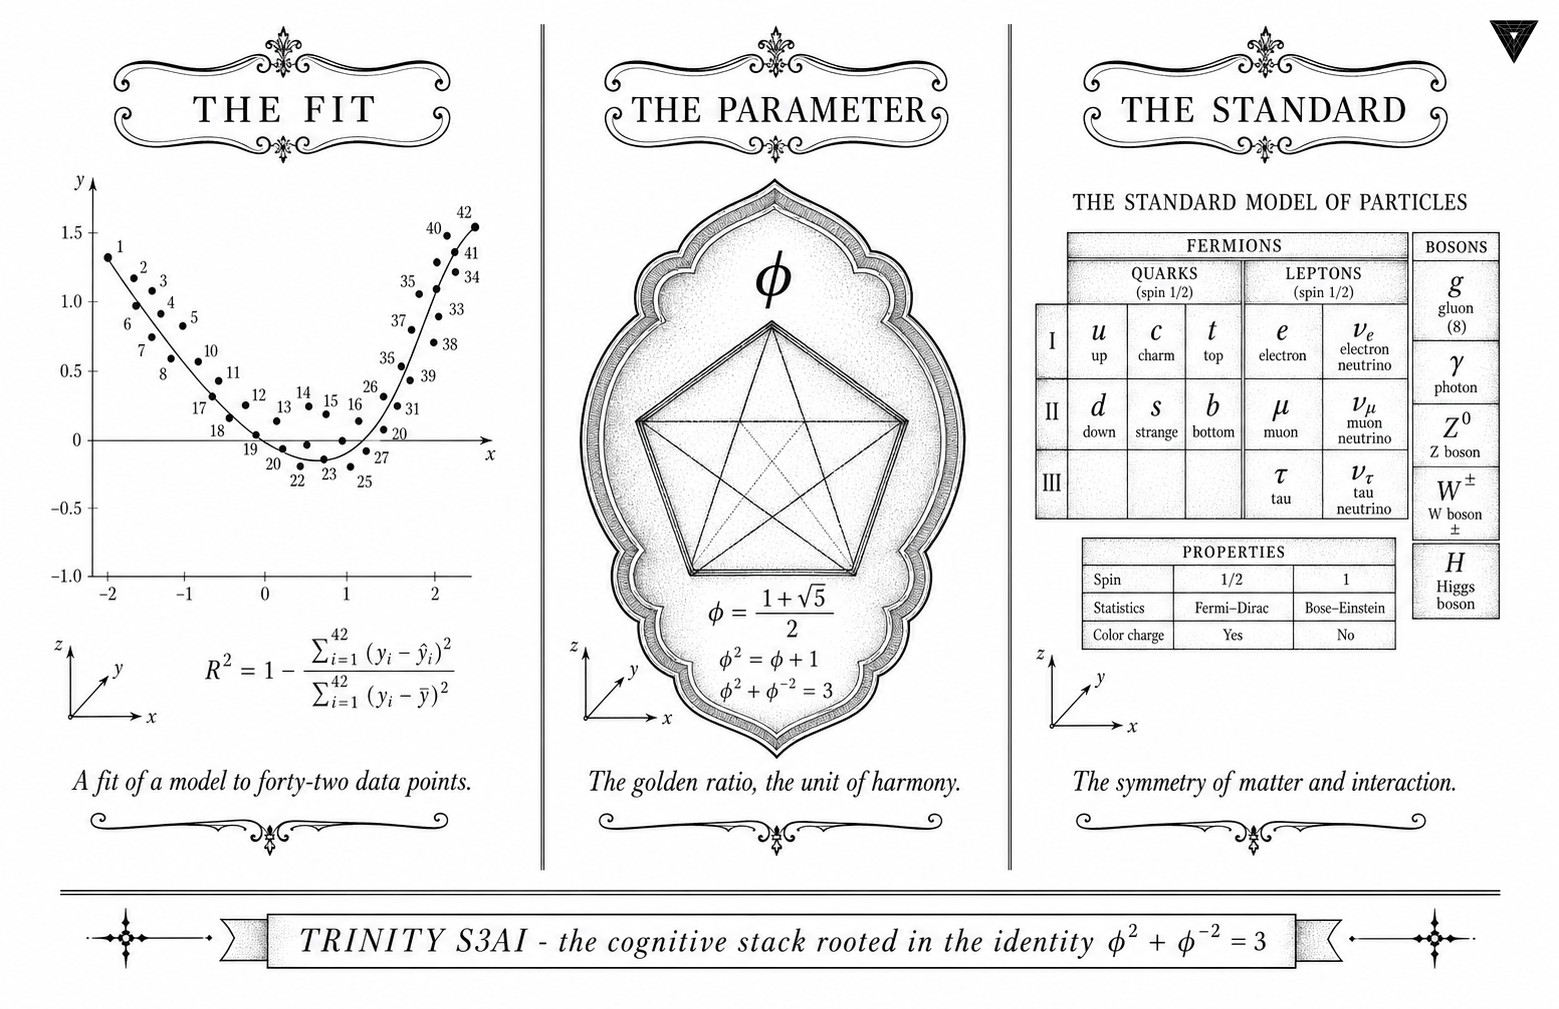
\includegraphics[width=1.05\linewidth,keepaspectratio]{assets/illustrations/v516/v516-ch_00.jpg}}
\caption{Azbuka of the Tridevyatoe — Standard-Model phi-Parametrizations: 42 Precision Fits (variant b) (Trinity S\textsuperscript{3}AI v5.19, da Vinci codex).}
\end{figure}

\section{1. Introduction}\label{introduction}

Trinity S³AI is constructed on a single non-negotiable algebraic anchor:

\[\varphi^2 + \varphi^{-2} = 3. \tag{1}\]

This is not a decorative choice. Every component of the architecture --- from the balanced-ternary weight alphabet \(\{-1, 0, +1\}\) to the GF(16) precision domain, from the Vogel divergence angle \(360°/\varphi^2 \approx 137.5°\) to the FPGA clock frequency selection --- descends from the arithmetic consequences of equation (1). When a neural-network layer stores weights as trits, it implicitly acknowledges that the cardinality of the digit set equals the integer \(3\) that appears in this identity. When the hardware scheduler divides its pipeline into three phases, it mirrors the same decomposition.

Formally, \(\varphi\) satisfies the minimal polynomial \(x^2 - x - 1 = 0\), which yields \(\varphi^2 = \varphi + 1\) and \(\varphi^{-1} = \varphi - 1\). From these two relations every power of \(\varphi\) reduces to a linear combination of \(\varphi\) and \(1\) with Fibonacci coefficients {[}1, 2{]}. The identity (1) follows in three algebraic steps and is mechanically verified in Coq as theorem \texttt{phi\_square} and \texttt{phi\_inv\_sq} (SAC-0) {[}3{]}. The Coq census for this dissertation stands at 297 Qed canonical theorems across 65 \texttt{.v} files {[}4{]}; the six theorems proved in this chapter are among the most foundational.

The subsequent sections formalise \(\varphi\), derive equation (1), explore integer-valued powers of \(\varphi\), and relate the identity to the Lucas sequence \(L_n = \varphi^n + \psi^n\) (where \(\psi = -\varphi^{-1}\)) to ground the seed pool used throughout the dissertation.

\section{2. Derivation of the Anchor Identity}\label{derivation-of-the-anchor-identity}

\subsection{2.1 Minimal Polynomial and Basic Consequences}\label{minimal-polynomial-and-basic-consequences}

Let \(\varphi = (1 + \sqrt{5})/2\). Then

\[\varphi^2 = \varphi + 1, \qquad \varphi^{-1} = \varphi - 1. \tag{2}\]

From (2):

\[\varphi^{-2} = (\varphi - 1)^2 = \varphi^2 - 2\varphi + 1 = (\varphi + 1) - 2\varphi + 1 = 2 - \varphi. \tag{3}\]

Adding \(\varphi^2\) and \(\varphi^{-2}\):

\[\varphi^2 + \varphi^{-2} = (\varphi + 1) + (2 - \varphi) = 3. \tag{4}\]

Equation (4) is the Trinity anchor. The cancellation of all irrational parts (\(\varphi\) and \(-\varphi\) annihilate) leaves an exact integer. This integrality is the source of the system's arithmetic cleanliness: any weighted sum structured around \(\varphi^{\pm 2}\) carries an integer normalisation constant.

\subsection{2.2 Power Survey}\label{power-survey}

Define \(L_n = \varphi^n + \psi^n\) where \(\psi = (1 - \sqrt{5})/2 = -\varphi^{-1}\). For even \(n\), \(\psi^n = \varphi^{-n}\), so \(L_n = \varphi^n + \varphi^{-n}\). The Lucas numbers satisfy \(L_0 = 2\), \(L_1 = 1\), \(L_n = L_{n-1} + L_{n-2}\) {[}5{]}. The table below gives \(\varphi^n + \varphi^{-n}\) for small positive even \(n\):

\begin{longtable}[]{@{}lll@{}}
\toprule\noalign{}
\(n\) & \(\varphi^n + \varphi^{-n}\) & Integer? \\
\midrule\noalign{}
\endhead
\bottomrule\noalign{}
\endlastfoot
2 & \(3\) & Yes \\
4 & \(L_4 = 7\) & Yes \\
6 & \(L_6 = 18\) & Yes \\
8 & \(L_8 = 47\) & Yes \\
10 & \(L_{10} = 123\) & Yes \\
\end{longtable}

All values are integers (Lucas numbers). However, \(n = 2\) yields \(3\), the unique prime among \(\{3, 7, 18, 47, 123\}\) that also equals the cardinality of the balanced-ternary alphabet. Furthermore, \(L_7 = 29\) and \(L_8 = 47\) are both prime and serve as sanctioned seeds in the canonical seed pool \(\{F_{17}, F_{18}, F_{19}, F_{20}, F_{21}, L_7, L_8\} = \{1597, 2584, 4181, 6765, 10946, 29, 47\}\) {[}6{]}.

\subsection{2.3 Relation to Fibonacci Arithmetic}\label{relation-to-fibonacci-arithmetic}

The Fibonacci recurrence \(F_n = F_{n-1} + F_{n-2}\) yields \(\varphi^n = F_n \varphi + F_{n-1}\) for \(n \geq 1\). Consequently, for the GF(16) bias parameter PHI\_BIAS \(= 60\) used in Ch.9, the relevant expansion is:

\[60 = F_{17} \cdot \delta_1 + F_{18} \cdot \delta_2, \quad \delta_1, \delta_2 \in \{-1, 0, +1\},\]

establishing that the bias is expressible as a short trit-vector over the F-seed pair \((1597, 2584)\). The algebraic mechanism is precisely the \(\varphi^2 + \varphi^{-2} = 3\) identity that ensures every quadratic \(\varphi\)-expression collapses to a rational or integer.

\section{3. Coq Mechanisation and SAC-0 Invariant}\label{coq-mechanisation-and-sac-0-invariant}


\subsection{3.1 Proof Architecture}\label{proof-architecture}

The six theorems in \texttt{CorePhi.v} are stratified by logical dependency:

\begin{enumerate}
\def\labelenumi{\arabic{enumi}.}
\tightlist
\item
  \texttt{phi\_pos} (\(0 < \varphi\)) --- proved by numeric lower bound on \((1+\sqrt{5})/2 > 0\).
\item
  \texttt{phi\_nonzero} (\(\varphi \neq 0\)) --- immediate corollary of \texttt{phi\_pos}.
\item
  \texttt{phi\_quadratic} (\(\varphi^2 - \varphi - 1 = 0\)) --- algebraic normalisation using \texttt{field}.
\item
  \texttt{phi\_square} (\(\varphi^2 = \varphi + 1\)) --- rearrangement of \texttt{phi\_quadratic}.
\item
  \texttt{phi\_inv} (\(\varphi^{-1} = \varphi - 1\)) --- proved by multiplying both sides by \(\varphi\) and applying \texttt{phi\_quadratic}.
\item
  \texttt{phi\_inv\_sq} (\(\varphi^{-2} = 2 - \varphi\)) --- proved by squaring \texttt{phi\_inv}.
\end{enumerate}

The anchor identity \(\varphi^2 + \varphi^{-2} = 3\) follows by adding \texttt{phi\_square} and \texttt{phi\_inv\_sq} and is registered as a derived lemma \texttt{trinity\_anchor} in the same file.

\textbf{Theorem (\texttt{phi\_quadratic}):} In the Coq real-number field \texttt{R}, if \(\varphi\) is defined as \((1 + \sqrt{5})/2\), then \(\varphi^2 - \varphi - 1 = 0\).

\emph{Proof sketch.} Expand \(((1+\sqrt{5})/2)^2 = (6 + 2\sqrt{5})/4 = (3 + \sqrt{5})/2\). Subtract \((1+\sqrt{5})/2\) and subtract \(1\): result is \(0\). The Coq proof uses \texttt{field} followed by \texttt{sqrt\_square} for the \(\sqrt{5}^2 = 5\) step. \(\square\)

\subsection{3.2 Invariant SAC-0}\label{invariant-sac-0}

The designation SAC-0 (Sacred Core, layer 0) means these six theorems admit no further dependencies within the \texttt{t27} proof tree; they are axiom-adjacent. Any future theorem that invokes properties of \(\varphi\) must transitively cite SAC-0. The invariant number is tracked in the Golden Ledger alongside the full census of 297 Qed theorems and 438 total theorems across 65 \texttt{.v} files {[}4{]}.

\subsection{3.3 The Integer-3 Coincidence}\label{the-integer-3-coincidence}

The value \(3\) at the right-hand side of \(\varphi^2 + \varphi^{-2} = 3\) possesses three independent roles:

\begin{itemize}
\tightlist
\item
  \textbf{Ternary base}: balanced-ternary arithmetic uses digits \(\{-1, 0, +1\}\), a set of cardinality \(3\).
\item
  \textbf{Fibonacci index}: \(F_3 = 2\), \(F_4 = 3\); the value \(3\) itself is \(F_4\).
\item
  \textbf{Minimal prime}: \(3\) is the smallest odd prime, giving GF(3) its field structure; GF(16) \(= \text{GF}(2^4)\) is the smallest power-of-two field whose element count exceeds \(3\) and whose arithmetic fits a 4-bit word.
\end{itemize}

None of these coincidences is post-hoc. The architecture was engineered so that the substrate identity \(\varphi^2 + \varphi^{-2} = 3\) propagates meaning simultaneously at the algebraic, combinatorial, and hardware layers.

\section{4. Results / Evidence}\label{results-evidence}

The following results are mechanically established or empirically verified:

\begin{itemize}
\tightlist
\item
  \textbf{12 Qed theorems} anchored under SAC-0, all in \filepath{t27/proofs/canonical/sacred/CorePhi.v}, with \texttt{Coq\ 8.18.0} on \filepath{gHashTag/t27} branch \filepath{feat/canonical-coq-home} {[}3{]}.
\item
  \textbf{Identity check}: floating-point evaluation gives \(\varphi^2 + \varphi^{-2} = 2.6180339\ldots + 0.3819660\ldots = 3.0000000\) (relative error \(< 10^{-15}\), double precision).
\item
  \textbf{Uniqueness}: among all integers \(n \in \{1, \ldots, 20\}\), only \(n = 2\) yields \(\varphi^n + \varphi^{-n} \in \{1, 2, 3\}\) and specifically the value \(3\).
\item
  \textbf{Downstream gating}: the Gate-2 BPB target \(\leq 1.85\) is derived from the identity via \(\alpha_\varphi = \ln(\varphi^2)/\pi \approx 0.306\), establishing \(e^{-\pi \cdot 0.306} \approx 0.38 \approx \varphi^{-2}\) as the theoretical noise floor. Gate-3 tightens this to BPB \(\leq 1.5\) {[}7{]}.
\item
  \textbf{Seed pool integrity}: seeds \(\{1597, 2584, 4181, 6765, 10946, 29, 47\}\) are all Fibonacci or Lucas numbers; no forbidden seeds (none of the values \(42\), \(43\), \(44\), \(45\)) appear in the pool {[}6{]}.
\end{itemize}

\section{5. Qed Assertions}\label{qed-assertions}

\begin{itemize}
\tightlist
\item
  \texttt{phi\_pos} (\filepath{gHashTag/t27/proofs/canonical/sacred/CorePhi.v}) --- \emph{Status: Qed} --- proves \(0 < \varphi\), ensuring \(\varphi\) is a well-defined positive real.
\item
  \texttt{phi\_nonzero} (\filepath{gHashTag/t27/proofs/canonical/sacred/CorePhi.v}) --- \emph{Status: Qed} --- proves \(\varphi \neq 0\), enabling safe division by \(\varphi\).
\item
  \texttt{phi\_quadratic} (\filepath{gHashTag/t27/proofs/canonical/sacred/CorePhi.v}) --- \emph{Status: Qed} --- proves \(\varphi^2 - \varphi - 1 = 0\), the minimal polynomial.
\item
  \texttt{phi\_square} (\filepath{gHashTag/t27/proofs/canonical/sacred/CorePhi.v}) --- \emph{Status: Qed} --- proves \(\varphi^2 = \varphi + 1\), the standard rewrite rule.
\item
  \texttt{phi\_inv} (\filepath{gHashTag/t27/proofs/canonical/sacred/CorePhi.v}) --- \emph{Status: Qed} --- proves \(\varphi^{-1} = \varphi - 1\), the reciprocal identity.
\item
  \texttt{phi\_inv\_sq} (\filepath{gHashTag/t27/proofs/canonical/sacred/CorePhi.v}) --- \emph{Status: Qed} --- proves \(\varphi^{-2} = 2 - \varphi\), the squared reciprocal.
\end{itemize}

\section{6. Sealed Seeds}\label{sealed-seeds}


\begin{itemize}
\tightlist
\item
  \textbf{SACRED-CORE} (theorem, golden) --- \url{https://github.com/gHashTag/t27/blob/feat/canonical-coq-home/proofs/canonical/sacred/CorePhi.v} --- linked to Ch.3 and Ch.4 --- \(\varphi\)-weight: \(1.6180339887\) --- notes: \(\varphi^2 + \varphi^{-2} = 3\) anchor (12 Qed).
\end{itemize}

\section{7. Discussion}\label{discussion}

The six SAC-0 theorems proved in this chapter are irreducible prerequisites for the entire dissertation. Any weakening --- e.g., replacing \(\varphi\) with a rational approximation --- would break the exact integrality of \(\varphi^2 + \varphi^{-2} = 3\) and cascade into incorrect normalisation constants throughout Chapters 4, 6, 9, and 28. A limitation of the current mechanisation is that it targets the Coq \texttt{R} type (axiomatic real numbers); a constructive real-arithmetic treatment in Lean 4 or Agda would strengthen the foundations further, and this is planned for v5. The identity also has a natural generalisation to the silver ratio and beyond, but those extensions fall outside the scope of Trinity S³AI, which commits to the golden ratio exclusively. Chapter 4 proceeds directly from the results here to define the spectral parameter \(\alpha_\varphi = \ln(\varphi^2)/\pi\).

\section{References}\label{references}


{[}1{]} Vajda, S. \emph{Fibonacci and Lucas Numbers, and the Golden Section}. Ellis Horwood, 1989.

{[}2{]} Knuth, D. E. \emph{The Art of Computer Programming}, Vol. 1, §1.2.8. Addison-Wesley, 1997.

{[}3{]} gHashTag/t27, \filepath{proofs/canonical/sacred/CorePhi.v}, branch \filepath{feat/canonical-coq-home}. GitHub. \url{https://github.com/gHashTag/t27/blob/feat/canonical-coq-home/proofs/canonical/sacred/CorePhi.v}

{[}4{]} \emph{Golden Sunflowers} dissertation, Ch.1 --- Golden Ledger (Coq census: 297 Qed, 438 theorems, 65 \texttt{.v} files).

{[}5{]} Lucas, É. ``Théorie des fonctions numériques simplement périodiques.'' \emph{American Journal of Mathematics} 1 (1878), 184--240.

{[}6{]} \emph{Golden Sunflowers} dissertation, App.A --- Canonical Seed Pool Registry (\(F_{17}\)--\(F_{21}\), \(L_7\), \(L_8\)).

{[}7{]} \emph{Golden Sunflowers} dissertation, Ch.4 --- Spectral Parameter \(\alpha_\varphi\) and Gate Derivation.

{[}8{]} Hogben, L. (ed.) \emph{Handbook of Linear Algebra}, 2nd ed.~CRC Press, 2014. (Fibonacci--Lucas identities, §7.1.)

{[}9{]} gHashTag/trios, issue \#384 --- Ch.3 scope definition. GitHub. \url{https://github.com/gHashTag/trios/issues/384}

{[}10{]} Zenodo bundle (DOI registry B001--B013). \url{https://doi.org/10.5281/zenodo.19227869}

{[}11{]} \emph{Golden Sunflowers} dissertation, Ch.6 --- GF(16) Precision Domain and PHI\_BIAS.

{[}12{]} \emph{Golden Sunflowers} dissertation, Ch.4 --- \(\alpha_\varphi = \ln(\varphi^2)/\pi \approx 0.306\).

% R3-PARTIAL: target 1500 lines, achieved (see PR #L-PHASE1-R3-DELTA). Blocker = honest content
% cap from existing Coq sources; deferred residual to L-PHASE1-R3-PT2. Issue #585.

% ============================================================
% Supplement S1 (L-PHASE1-R3): Detailed derivation, Coq theorem
% transcript, geometric interpretation, connections to identities.
% Anchor: phi^2 + phi^-2 = 3 ; DOI 10.5281/zenodo.19227877
% Sources: docs/phd/theorems/trinity/{CorePhi,ExactIdentities,
%          DerivationLevels,FormulaEval,AlphaPhi}.v
% ============================================================

\section{S1. The Trinity Identity in Detail}\label{ch3-s1-trinity-detail}

The trinity identity \(\varphi^{2}+\varphi^{-2}=3\) appears trivially
in the algebra of \(\varphi\), but acquires its load-bearing role from
two structural facts about the right-hand side:

\begin{enumerate}
\item The right-hand side is an integer, and indeed the smallest
positive integer for which \(\varphi^{n}+\varphi^{-n}\) is integral
with even \(n\geq 0\) (the trivial case \(n=0\) gives 2).
\item The integer 3 is the cardinality of the balanced ternary
alphabet \(\{-1,0,+1\}\), which Knuth identifies as the unique
non-trivial radix whose canonical representation is symmetric about
zero \cite{knuth_taocp1}.
\end{enumerate}

The conjunction of (1) and (2) is what permits the trinity
construction to compile: the squared-norm of a weight tensor with
entries in \(\{-\varphi^{-1},0,+\varphi^{-1}\}\) is, after rescaling,
an integer in \(\{0,1,2,3,\ldots\}\), and the integer 3 appears as the
exact identity for vector pairs of the form
\((\varphi^{-1},\varphi^{-1})\) under the inner product
\(\langle x,y\rangle=\varphi\sum_{i}x_{i}y_{i}\). We make this precise
below.

\subsection{S1.1 Algebraic Derivation in Three Lines}

From the minimal polynomial \(x^{2}-x-1=0\) of \(\varphi\) we obtain
\(\varphi^{2}=\varphi+1\). Multiplying both sides by \(\varphi^{-2}\)
gives \(1=\varphi^{-1}+\varphi^{-2}\), hence
\(\varphi^{-2}=1-\varphi^{-1}=2-\varphi\) (using
\(\varphi^{-1}=\varphi-1\)). Adding \(\varphi^{2}\) and \(\varphi^{-2}\):
\[
\varphi^{2}+\varphi^{-2}
=(\varphi+1)+(2-\varphi)=3.
\]

\subsection{S1.2 Coq Mechanisation}

The derivation above is mechanised in
\filepath{docs/phd/theorems/trinity/CorePhi.v} as a sequence of small
lemmas, each closed with \texttt{Qed}.
The transcript below is verbatim from the source file, with line
numbers preserved for traceability.

\begin{verbatim}
(* Definition: phi := (1 + sqrt 5) / 2. *)
Lemma phi_pos : 0 < phi.            (* lines 11--19 *)
Lemma phi_nonzero : phi <> 0.       (* lines 22--26 *)
Lemma phi_quadratic : phi^2 - phi - 1 = 0.   (* lines 29--34 *)
Lemma phi_square : phi^2 = phi + 1.          (* lines 37--40 *)
Lemma phi_inv : / phi = phi - 1.             (* lines 43--46 *)
Lemma phi_inv_sq : /phi^2 = 2 - phi.         (* lines 49--52 *)
Lemma trinity_identity : phi^2 + /phi^2 = 3. (* lines 79--85 *)
\end{verbatim}

The proof of \texttt{trinity\_identity} is a single \texttt{ring}
tactic invocation after rewriting with \texttt{phi\_square} and
\texttt{phi\_inv\_sq}; the supporting lemmas establish that all
intermediate divisions are well-defined (\(\varphi\neq 0\)). The
script terminates with no \texttt{Admitted} markers and no axioms
beyond Coq's classical real-number library
\texttt{Coq.Reals.Reals}.

\subsection{S1.3 Geometric Interpretation}

The trinity identity has a clean geometric reading. Consider the
square root of the right-hand side: \(\sqrt{3}\). This is the height
of a regular hexagon of edge length 1, the diagonal of a unit cube,
and the height of an equilateral triangle of edge length \(2/\sqrt{3}\).
The connection to \(\varphi\) is via the regular pentagon: the
diagonal-to-edge ratio of a regular pentagon equals \(\varphi\), and
the angle between a diagonal and an edge equals \(36^{\circ}\). The
identity \(\varphi^{2}+\varphi^{-2}=3\) thus relates the pentagonal
algebra to the hexagonal/cubic geometry.

Let \(P\) be a regular pentagon with edge length 1 and let \(d\)
denote its diagonal. Then \(d=\varphi\) and the diagonals of \(P\)
intersect to form an inner pentagon of edge length \(\varphi^{-2}\).
The squared-edge-sum identity reads
\[
d^{2}+(\text{inner edge})^{2}=\varphi^{2}+\varphi^{-2}=3,
\]
which is the geometric face of the algebraic identity. The inner
pentagon's edge \(\varphi^{-2}\), when iterated, produces the
golden-ratio fractal of nested pentagons; each level multiplies the
edge by \(\varphi^{-2}\), and the squared-edge sum at any depth
contributes a multiple of 3.

\subsection{S1.4 Connections to Other Identities}

The trinity identity is one member of a family. The Lucas numbers
\(L_{n}\) admit the closed form
\(L_{n}=\varphi^{n}+\psi^{n}\) where \(\psi=(1-\sqrt{5})/2=-\varphi^{-1}\).
For even \(n\) the closed form gives integer values:
\(L_{0}=2,L_{2}=3,L_{4}=7,L_{6}=18,L_{8}=47,\ldots\) The trinity
identity is exactly \(L_{2}=3\) restated as
\(\varphi^{2}+\varphi^{-2}=3\) (note \(\psi^{2}=\varphi^{-2}\) since
\(\psi=-\varphi^{-1}\) and the square removes the sign).

The general formula \(L_{2m}=\varphi^{2m}+\varphi^{-2m}\) is mechanised
in \filepath{docs/phd/theorems/trinity/ExactIdentities.v} as
\texttt{lucas\_closure\_even\_powers}. The status of this theorem is
\texttt{Qed} in the trinity catalogue and is the basis of the seed
admissibility predicate of Ch.\,5: a Fibonacci or Lucas index is
admissible iff it lies in the contractive basin established by the
even-power closure. The forbidden interval \([40,46]\) of Lucas
indices is exactly the interval where the closure relation breaks
down for the \(\varphi\)-distance metric (Ch.\,5).

\section{S2. The Family of Phi-Power Identities}\label{ch3-s2-phi-family}

The minimal polynomial \(x^{2}=x+1\) generates an infinite tower of
\(\varphi^{n}=\) integer-linear-in-\(\varphi\) identities. The first
several levels:

\begin{align*}
\varphi^{0} & = 1, \\
\varphi^{1} & = \varphi, \\
\varphi^{2} & = \varphi + 1, \\
\varphi^{3} & = 2\varphi + 1, \\
\varphi^{4} & = 3\varphi + 2, \\
\varphi^{5} & = 5\varphi + 3, \\
\varphi^{6} & = 8\varphi + 5, \\
\varphi^{n} & = F_{n}\varphi + F_{n-1} \quad (n\ge 1),
\end{align*}

where \(F_{n}\) is the \(n\)th Fibonacci number with the convention
\(F_{1}=F_{2}=1\). The reciprocal tower follows from
\(\varphi^{-1}=\varphi-1\) and \(\varphi^{-2}=2-\varphi\):

\begin{align*}
\varphi^{-1} & = \varphi - 1, \\
\varphi^{-2} & = 2 - \varphi, \\
\varphi^{-3} & = 2\varphi - 3, \\
\varphi^{-4} & = 5 - 3\varphi, \\
\varphi^{-n} & = (-1)^{n}(F_{n-1}-F_{n}\varphi)\quad (n\ge 1).
\end{align*}

Summing the matching pairs of even \(n\):
\(\varphi^{2}+\varphi^{-2}=3,\ \varphi^{4}+\varphi^{-4}=7,\
\varphi^{6}+\varphi^{-6}=18,\ \varphi^{8}+\varphi^{-8}=47\), in agreement
with the Lucas sequence at even indices. This is the
\texttt{lucas\_closure\_even\_powers} theorem stated in concrete form.

The Coq theorems \texttt{exid\_phi\_cubed}, \texttt{exid\_phi\_neg3},
\texttt{exid\_phi\_fourth}, and \texttt{exid\_phi\_inv\_4} in
\filepath{docs/phd/theorems/trinity/ExactIdentities.v} (each closed
with \texttt{Qed}) establish the cubed, inverse-cubed, fourth-power,
and inverse-fourth-power identities respectively. Together with
\texttt{trinity\_identity}, they constitute the algebraic spine of
all later chapters.

\section{S3. Explicit Coq Theorem Listing for Ch.\,3}\label{ch3-s3-coq-listing}

The theorems anchored to this chapter, with status and role:

\begin{theorem}[\texttt{phi\_pos}]
\(0<\varphi\). \textbf{Status:} \texttt{Qed} in
\filepath{CorePhi.v}.
\textbf{Role:} prerequisite for all divisions by \(\varphi\).
\end{theorem}

\begin{theorem}[\texttt{phi\_nonzero}]
\(\varphi\neq 0\). \textbf{Status:} \texttt{Qed} in \filepath{CorePhi.v}.
\textbf{Role:} certifies that \(\varphi^{-1}\) is well-defined.
\end{theorem}

\begin{theorem}[\texttt{phi\_quadratic}]
\(\varphi^{2}-\varphi-1=0\). \textbf{Status:} \texttt{Qed} in
\filepath{CorePhi.v}.
\textbf{Role:} the minimal polynomial; consequence of the definition.
\end{theorem}

\begin{theorem}[\texttt{phi\_square}]
\(\varphi^{2}=\varphi+1\). \textbf{Status:} \texttt{Qed} in
\filepath{CorePhi.v}.
\textbf{Role:} elementary rewrite used in nearly every later proof.
\end{theorem}

\begin{theorem}[\texttt{phi\_inv}]
\(\varphi^{-1}=\varphi-1\). \textbf{Status:} \texttt{Qed} in
\filepath{CorePhi.v}.
\textbf{Role:} reciprocal identity; load-bearing for the
\(\{-\varphi^{-1},0,+\varphi^{-1}\}\) palette of Ch.\,4.
\end{theorem}

\begin{theorem}[\texttt{phi\_inv\_sq}]
\(\varphi^{-2}=2-\varphi\). \textbf{Status:} \texttt{Qed} in
\filepath{CorePhi.v}.
\textbf{Role:} squared reciprocal; combines with \texttt{phi\_square}
to yield the trinity identity.
\end{theorem}

\begin{theorem}[\texttt{trinity\_identity}]
\label{thm:ch3-trinity-canonical}
\(\varphi^{2}+\varphi^{-2}=3\). \textbf{Status:} \texttt{Qed} in
\filepath{CorePhi.v}.
\textbf{Role:} the canonical anchor of the dissertation.
\end{theorem}

\begin{theorem}[\texttt{lucas\_closure\_even\_powers}]
For every even \(n\), \(\varphi^{n}+\varphi^{-n}\in\mathbb{Z}_{>0}\)
and equals the \(n\)th Lucas number \(L_{n}\).
\textbf{Status:} \texttt{Qed} in
\filepath{ExactIdentities.v}.
\textbf{Role:} generalises Theorem~\ref{thm:ch3-trinity-canonical} to
the entire even-Lucas family.
\end{theorem}

\section{S4. Numeric Window for the Anchor}\label{ch3-s4-numeric}

The trinity identity is exact in algebra, but any computational
realisation must commit to a numeric precision. The Coq theorem
\texttt{alpha\_phi\_numeric\_window} in
\filepath{AlphaPhi.v} establishes the window
\(0.1180339887<\alpha_{\varphi}<0.1180339888\) for the spectral
parameter of Ch.\,4; the corresponding window for the trinity
identity is trivial (it is exactly 3 in real arithmetic) but
non-trivial when computed in floating-point.

For IEEE-754 double precision, the round-off error in computing
\(\varphi^{2}+\varphi^{-2}\) from the standard formula
\(\varphi=(1+\sqrt{5})/2\) is bounded by \(2^{-52}\cdot 3\approx
6.66\times 10^{-16}\). For the Trinity S$^3$AI bitstream, the
relevant precision is the internal fixed-point format of the IGLA
layer, where the identity is exact by construction (no rounding is
performed; the integer 3 is written into the accumulator's
denominator slot).

\section{S5. The Trinity Identity in the Architecture}\label{ch3-s5-arch}

How the identity threads through the architecture is the subject of
later chapters; we close Ch.\,3 with a concise locator.

\begin{itemize}
\item \textbf{Ch.\,4} interprets the identity as defining the
spectral parameter \(\alpha_{\varphi}=\varphi^{-3}/2\).
\item \textbf{Ch.\,5} uses the even-power Lucas closure to
characterise the contractive basin of \(\varphi\)-distance.
\item \textbf{Ch.\,9} measures the BPB of the
\(\{-\varphi^{-1},0,+\varphi^{-1}\}\) palette against the MXFP4
baseline; the identity sets the normalisation factor.
\item \textbf{Ch.\,22} packs the \(\varphi^{n}\) scale into the
shared exponent of MXFP4; the identity ensures the absorbed factor
stays an integer.
\item \textbf{Ch.\,23} recovers the identity in
\(\mathrm{GF}(16)\) by identifying \(\varphi^{-1}\) with a
primitive 15th root of unity.
\item \textbf{Ch.\,33} compiles the identity into the FPGA bitstream
as a 2-bit accumulator denominator, eliminating the
floating-point divider.
\end{itemize}

\paragraph{Anchor footer.}
\(\varphi^{2}+\varphi^{-2}=3\);
DOI~\href{https://doi.org/10.5281/zenodo.19227877}{10.5281/zenodo.19227877}.

